\chapter{Controlador de corriente} \chapterlabel{Informe/4-ControladorCorriente} \label{cap:ControladorCorriente}

En este capítulo se diseña y modela el circuito encargado de controlar la corriente que circula por el electroimán. Como se vio en el capítulo anterior, el sistema trabaja con corrientes elevadas por lo que se implementan estrategias de conmutación para reducir las pérdidas de energía. Para ello se utiliza una topología de puente H con cuatro MOSFET y un \textsl{driver} que los controla. Además, se detallan los criterios tenidos en cuenta al momento de  elegir  y dimensionar todos los componentes que intervienen para lograr el correcto funcionamiento del controlador de corriente. Por último, se obtiene su función transferencia  para ser utilizada en el diseño del compensador.

\section{Descripción general}

Para mantener en suspensión a la pieza móvil es necesario regular la fuerza electromagnética generada por el electroimán. Esto se logra modificando la intensidad de la corriente que circula por su bobinado. Para ello, es necesario diseñar una fuente de alimentación que sea capaz de proveer la corriente requerida.

Para diseñar la fuente de alimentación se debe conocer el comportamiento eléctrico de la planta. Como se analizó en el capítulo \ref{cap:CaracterizacionElectroiman}, el electroimán puede ser modelado como una inductancia variable con una resistencia serie. Es decir, es un circuito RL serie cuya corriente ($I_L$) depende de la tensión aplicada ($V_L$). La expresión \ref{eq_corriente} muestra la relación entre estos parámetros.

\begin{equation} \label{eq_corriente}
\frac{I_L}{V_L}(s)=\frac{1}{sL(Y_g)\ +\ R_L}
\end{equation}

Al aplicar la transformada inversa de Laplace a la expresión  \ref{eq_corriente}, se puede obtener la respuesta temporal de la corriente ante un escalón de tensión de amplitud ``$v_L$'' en la entrada:

\begin{equation} \label{eq_corriente_temporal}
	i_L(t)=\frac{v_L}{R_L}*(1-\frac{1}{L(Y_g)}*e^{-\frac{R_L}{L(Y_g)}*t})
\end{equation}

\colorbox{red}{revisar lo de arriba}En la expresión \ref{eq_corriente_temporal} se puede observar que la respuesta al escalón está compuesta por dos partes: un término con una exponencial negativa correspondiente al transitorio, y un término constante correspondiente al valor en régimen permanente $\frac{v_L}{R_L}$. El primero provoca que la corriente en el inductor crezca de manera amortiguada, hasta alcanzar el valor de régimen permanente luego de cierto tiempo. Este comportamiento se puede observar en la simulación realizada en la figura \ref{fig:img_respuesta_escalon}. En la parte superior de la figura se observa la tensión de entrada, y en la parte inferior la corriente del electroimán. Este análisis resulta de utilidad para conocer el comportamiento del electroimán y diseñar un controlador de corriente adecuado.


\begin{figure}[H]
	\centering
	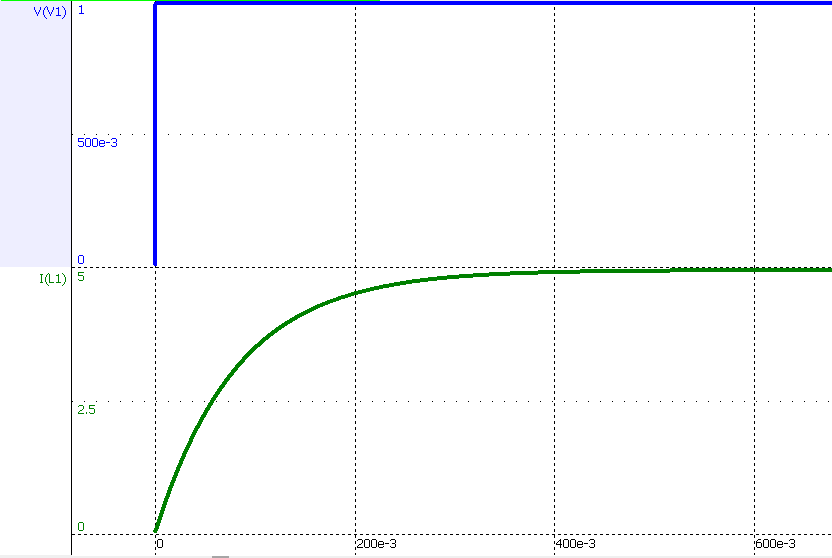
\includegraphics[scale=0.5]{corriente_escalon.png}
	\caption{Respuesta ante una entrada en escalón.}
	\label{fig:img_respuesta_escalon}
\end{figure}


\section{Diseño de topología}


Se desea diseñar un sistema de control que modifique la alimentación del electroimán con el objetivo de que circule una corriente específica por su bobinado.  Para ello, se implementa un sistema realimentado que compara la corriente que circula por el electroimán con una de referencia, que es la que se desea que circule por el electroimán. En la figura \ref{fig:img_diagrama_bloques_basico} se muestra un diagrama en bloques inicial del sistema.


\begin{figure}[H]
	\centering
	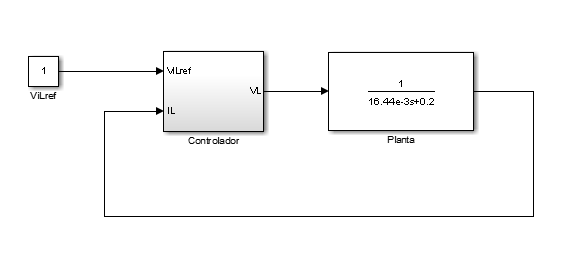
\includegraphics[scale=1]{Diagrama-en-bloques-basico.png}
	\caption{Diagrama en bloques básico del controlador de corriente.}
	\label{fig:img_diagrama_bloques_basico}
\end{figure}

\colorbox{red}{Acá estaría bueno proponer} que vamos a analizar dos manera de controlar la corriente. o alguna intro similar

\subsection{Control de corriente mediante transistor en modo lineal}

Como se vio en la introducción del capítulo, el valor en régimen permanente de la corriente depende proporcionalmente de la tensión aplicada al electroimán. Por lo tanto, 

Para mantener una corriente constante controlada se podría utilizar un transistor en modo lineal, es decir, como una fuente de corriente constante. Una posible implementación circuital se muestra en la figura \ref{fig:img_controlador-lineal}.

\begin{figure}[H]
	\centering
	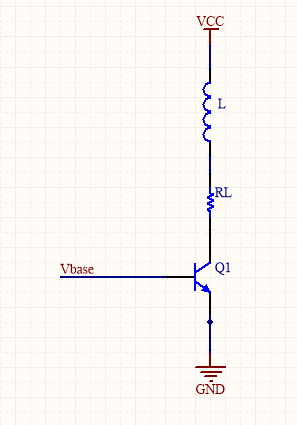
\includegraphics[scale=0.7]{controlador_lineal.png}
	\caption{Control de corriente mediante transistor en modo lineal.}
	\label{fig:img_controlador-lineal}
\end{figure}

En este modo de funcionamiento la tensión colector-emisor ($V_{CE}$) se controla de manera que la diferencia entre esta y la tensión de alimentación, circulando por la resistencia interna del electroimán, generen la corriente deseada. Es decir, en régimen permanente se obtiene:
 
 \begin{equation} \label{eq_corriente_temporal}
 	I_L=\frac{V_{CC}-V_{CE}}{R_L}
 \end{equation}
 
La desventaja de esto es que al circular una corriente constante, la caída de tensión sobre el inductor es prácticamente nula (solo lo correspondiente a la resistencia interna). Por lo tanto, la mayor parte de la potencia disipada cae sobre el transistor. Esta puede calcularse como: 

\begin{equation}
	P_{transistor} = I_L*V_{CE}
\end{equation}

Teniendo en cuenta que la tensión colector-emisor es la resta de la tensión de alimentación y la caida en la resistencia del electroimán:

\begin{equation}
	V_{CE}=V_{CC}-I_L*R_L
\end{equation}

Finalmente:

\begin{equation}
	P_{transistor}=V_{CC}*I_L-I_L^2*R_L
\end{equation}

Esta función llega a un máximo cuando $I_L=\frac{V_{CC}}{2*R_L}$


\begin{equation}\label{eq_pot_transistor_lineal_final}
	P_{transistor_{max}}=\frac{V_{CC}^2}{4*R_L}
\end{equation}

Teniendo en cuenta que la corriente maxima que se requiere es de aproximadamente 30 A se puede obtener que la minima tension de VCC requerida es:

\begin{equation}
	V_{CC}=I_L*R_L+V_{CE}=30 A * 0,2  = 5 V, VCE=0
\end{equation}

En el mercado las fuentes de tension capaces de entregar 30 A mas comunes en el mercado comienzan con valores minimos de 12 V. Si se reemplaza este valor en la ecuacion  \ref{eq_pot_transistor_lineal_final} se obtiene un valor minimo de 180 Watt, esto elevaria demasiado la temperatura del transistor, haciendo que sea necesario el agregado de un gran disipador de calor y pone en riesgo la vida útil de los componentes.
  
En la ecuaicion \ref{eq_pot_transistor_lineal_fina} se puede ver que para valores de tension normalmente utilizados $(5\:V,10\:V,15\:V)$ la potencia disipada por el transistor varía entre $30\:W$ hasta $280\:W$. Esto eleva demasiado la temperatura del transistor, haciendo que sea necesario el agregado de un gran disipador de calor y pone en riesgo la vida útil de los componentes.

Aunque aún no se define con qué tensión se alimentará el sistema, se puede probar con valores utilizados comunmente para obtener una aproximación de la potencia disipada por el transistor. Por ejemplo, para valores de tensión de alimentación $(5\:V,10\:V,15\:V)$ el valor de potencia que se obtiene varía entre $30\:W$ hasta $280\:W$. Esto eleva demasiado la temperatura del transistor, haciendo que sea necesario el agregado de un gran disipador de calor y pone en riesgo la vida útil de los componentes.

\colorbox{red}{HACER UN MEJOR ENGANCHE}

\subsection{Control de corriente mediante conmutación}

Como se analizó en la sección anterior, al trabajar con corrientes elevadas, no es eficiente utilizar un transistor que trabaje en su zona lineal puesto que el consumo de energía es elevado. Se propone entonces utilizar una fuente conmutada.

\noindent Para lograr una corriente contínua en el electroimán mediante una fuente conmutada se debe alternar la polaridad de la tensión aplicada en los bornes del inductor. De esta forma, la corriente crece y decrece (según la polaridad de tensión aplicada) en torno al valor medio deseado con forma exponencial debido a la resistencia interna del electroimán. Sin embargo, como el intervalo de tiempo de esta conmutación es pequeño comparado con la constante de tiempo de la planta, el incremento de corriente será pequeño y puede ser aproximado a una recta. Por lo tanto, se obtiene una corriente contínua con un ripple superpuesto de forma triangular, como la que se muestra en la figura \ref{fig:img_corriente_triangular_2}. 

\begin{figure}[H]
	\centering
	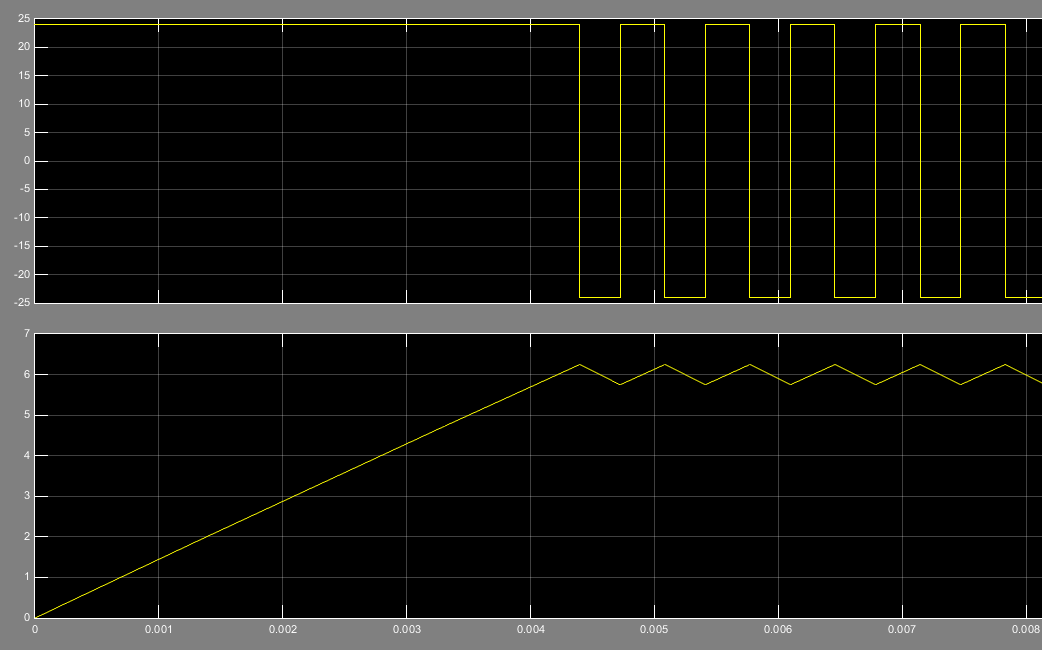
\includegraphics[scale=0.5]{corriente_triangular.PNG}
	\caption{Forma de onda de corriente.}
	\label{fig:img_corriente_triangular_2}
\end{figure}


\noindent Para lograr alternar la polaridad de la fuente sobre el inductor se utiliza una topología en puente H con cuatro llaves como se  muestra en la figura.

\begin{figure}[H]
	\centering
	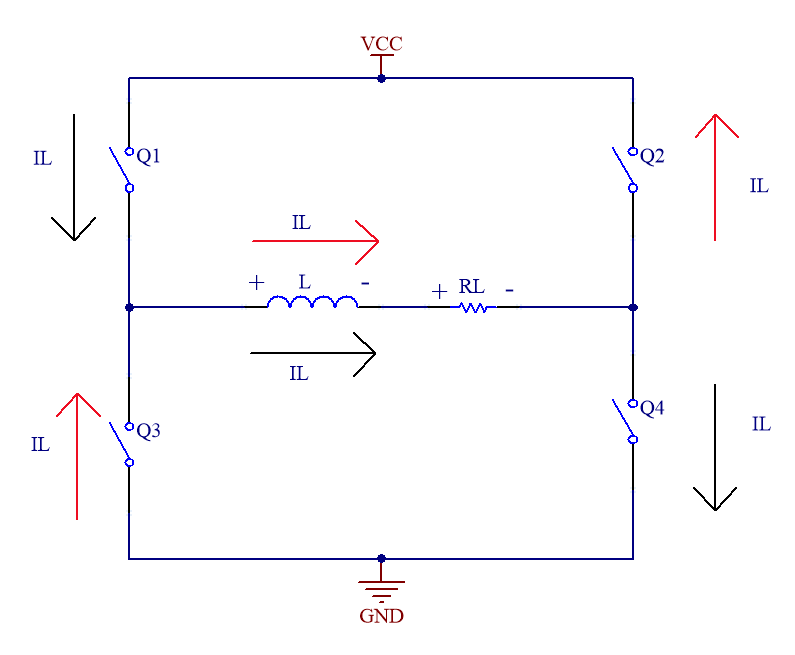
\includegraphics[scale=0.5]{puente_con_llaves.png}
	\caption{Topología simplificada.}
	\label{fig:img_topologia_simplificada}
\end{figure} 
\colorbox{red}{Agregar nombres a las llaves (Q1,Q2,Q3,Q4)}

El electroimán se conecta entre los puntos medios de cada par de llaves. De esta manera se puede conmutar la polaridad de la tensión que se le aplica. Sólo se permite que dos llaves se enciendan a la vez, y esto se realiza de manera diagonal. Es decir, en la figura \ref{fig:img_topologia-puenteH}, $Q_1$ y $Q_4$ pueden estar encendidos, mientras que $Q_3$ y $Q_2$ están apagados, y viceversa. De otra forma, se podría generar un cortocircuito entre la fuente de alimentación y GND, que produciría una circulación de corriente denominada \textsl{shoot-through}.

Para poder generar una corriente triangular con un valor medio deseado es necesario controlar el tiempo que se le aplica cierta polaridad de tensión al electroimán. Para poder controlar dicha polaridad, se debe actuar sobre las llaves en función de si se desea aumentar o disminuir el valor medio de la corriente. 

Una manera de hacerlo es mediante un circuito que compare la corriente de referencia con la corriente que está circulando por el electroimán. De esta forma, si la corriente es menor a la de referencia, la polaridad de la tensión aplicada en los bornes del electroimán, será positiva. En cambio, si resulta mayor, será negativa. De esta forma, la corriente aumenta y disminuye respectivamente. 

Con el circuito planteado hasta ahora, una vez que la corriente del electroimán supere infinitesimalmente a la referencia, se produciría una conmutación en la polaridad de tensión aplicada al electroimán. Lo mismo sucedería cuando sea infinitesimalmetne menor. Esto produciría conmutaciones extremadamente rápidas en torno al valor medio y sería necesario alta velocidad en conmutación. Por lo tanto, para evitar esas oscilaciones, es necesario agregar un retraso de tiempo para evitar que la fuente conmute de forma indeseada.

Una manera de hacerlo es mediante un comparador con histéresis. Este bloque compara la corriente de referencia con la que está circulando por el electroimán y permite definir un ancho de histeresis. De esta forma en caso de que esta última sea menor que la referencia, la polaridad de tensión aplicada al electroimán será positiva y, por ende, la corriente aumentara hasta alcanzar la referencia. Una vez superada la referencia, se volverá a cambiar la polaridad en el electoimán, pero esta vez será negativa, haciendo que el valor medio de la corriente disminuya. Debido a que lo unico que cambia es el valor de tension en modulo con el que se exita al electroiman la constante de tiempo del circuito no cambia. Esto da como resultado a que la corriente oscile sobre un valor medio de forma triangular. El valor de el ripple de corriente esta determinado por el periodo de conmutacion de la fuentes. Estos parametros pueden ser definidos ajustando el ancho de histeresis...

en este tipo de fuentes, la manera de lograr una corriente continua en un inductor es generando una onda triangular cuyo valor medio sea el valor de contìnua deseado, y que tenga una variaciòn pequeña alrededor de este. 
+
PONEMOS IMAGEN TRIANGULAR
Se desea controlar el valor medio de la corriente que circula por el bobinado del electoimán. Sabiendo que al aplicar una tensión constante en sus terminales la magnitud de la corrietne crece, se propone diseñar una fuente conmutada, de forma tal qeu una vez alcanzada el valor medio de corriente deseado, se pueda alternar la polaridad 

Otra estrategia es trabajar en conmutación como se muestra en la figura dasd.

Esta topología permite alternar...

Otra forma de controlar la corriente sobre un inductor es la de conmutar sobre sus bornes la tensión de alimentación. De esta forma se puede lograr una forma de onda triangular de corriente con un valor medio como se muestra en la figura XD. Ademas,

IMAGEN DE ONDA TRIANGULAR CON VALOR MEDIO Capaz q otra mas piola.


\begin{equation}
V_{L} =L*\frac{di}{dt}
\end{equation}

\begin{equation}
i =\frac{1}{L}\int{V(x)*dx}+i(0) , i(0)=0
\end{equation}

\begin{equation}
Potencia_{inductor} = V*I_{max}=RL*I_{max}^2=\frac{RL}{L}*(\int{V(x)*dx})^2=\frac{RL}{L}*\frac{T*V_{conm}}{4*L}
\end{equation}

\begin{equation}
Potencia_{inductor} = V*I_{max}=L_{max}*i_{max}*\frac{di}{dt}
\end{equation}

NOSE SI ESTAN BIEN LAS EQ, Pero si estan se podria decir algo como que si se eligen bien ciertos parametros(Tiempo de conmutacion[T] y Vconmutacion) se puede reducir el consumo de potencia xq hay cosas como L, RL e imax que ya sabemos cuanto valen

Como se puede ver en la imagen xd, el incremento y decremento de la corriente está definido por los tiempos de conmutación. Por lo tanto al actuar sobre estos tiempos se pueden ajustar el valor medio y el ripple que tendrá la corriente de la forma que se desea. Para lograr esto se debe tener conocimiento de que estado tiene la corriente, por lo tanto se plantea un diagrama en bloques con un bloque principal de conmutación, la planta, y agrega una realimentación de la corriente.



Para generar la corriente deseada en el inductor se puede proceder de la siguiente manera:

\begin{itemize}
\item En primer lugar, se inicia con corriente nula en el inductor. Se conecta alimentación sobre el inductor en sentido positivo y la corriente comienza a crecer con forma de rampa.
\item Se debe tomar medición de esta corriente, para que al superar el valor medio deseado + ripple/2, se debe invertir la polaridad de la alimentación.
\item La corriente comienza a decrecer. Cuando llega al valor medio deseado - ripple/2, se vuelve a invertir la polaridad y la corriente vuelve a crecer. De manera que se repite el ciclo y se obtiene una forma de onda triangular.
\end{itemize}

Para lograr esto se realimenta la corriente del electroimán a un comparador. Este circuito compara dos señales V1 con V2 y dependiendo del resultado de dicha comparación se obtiene una salida. Al realimentar la corriente se puede determinar si el circuito 
Se dice que el comparador tiene histéresis porque



Se desea diseñar un sistema de control que modifique la alimentación del electroimán, con el objetivo de que su corriente siga de manera proporcional a una tensión de referencia que entra al controlador. Es decir, se quiere un diagrama en bloques como: 

\begin{figure}[H]
	\centering
	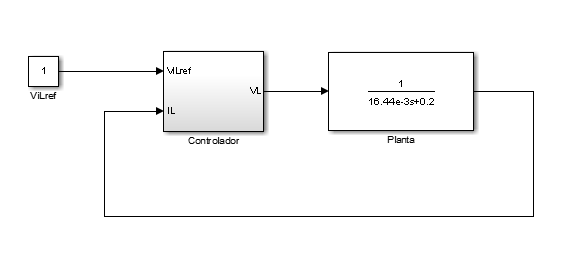
\includegraphics[scale=1]{Diagrama-en-bloques-basico.png}
	\caption{Diagrama en bloques básico del controlador. IGUAL YA ESTAMOS SPOILEANDO QUE SE REALIMENTA}
	\label{fig:img_diagrama_bloques_basico}
\end{figure}

Con el resultado de la descripción general se podría pensar en que para obtener un valor de corriente deseado, se debería controlar la tensión de alimentación del electroimán... ACÁ QUERÍA DECIR QUE SE PODRÍA HACER UN CONTROLADOR LINEAL CON UN TRANSISTOR PERO QUE ES MALA IDEA POR LA DISIPACIÓN 

\colorbox{red}{hasta acá hice}

\noindent Se desea controlar la corriente que circula por el electroimán y, debido a que el sistema va a trabajar con corrientes elevadas, es importante que la implementación del controlador de corriente sea eficiente. Por lo tanto, para disminuir la disipación de potencia del circuito se utiliza un controlador que funciona en conmutación.

\colorbox{red}{lo escribiría como:}
Se desea entonces diseñar un circuito que le brinde al electroimán la alimentación adecuada para que por su bobinado circule una corriente contínua de un valor que pueda ser controlado de manera externa (mediante una tensión de referencia).

De la ecuación \ref{eq_admitancia} se puede observar que la corriente en el electroimán sufre un transitorio en forma de exponencial creciente para luego estabilizarse en un valor V/R en régimen permanente. La solución mas simple que se podría idear es la de utilizar un circuito que varíe la alimentación del electroimán. ¿como se logra esto? Si se tiene una fuente de alimentación fija para todo el circuito y se desea obtener una tensión variable en el bobinado, se podría implementar un circuito con un transistor funcionando en zona lineal y variar su tensión colector-emisor. \colorbox{red}{poner figura ejemplo}

Este circuito podría funcionar pero tiene la desventaja de que debido a que el sistema trabaja con corrientes elevadas se producen grandes pérdidas de energía en el transistor. 

Debido a que el sistema va a funcionar con corrientes elevadas, es importante minimizar las pérdidas de energía que puedan ocurrir en la circuitería del controlador de corriente. Por lo tanto, se debería implementar un controlador que trabaje en conmutación.  En este tipo de controladores se aprovecha el transitorio de corriente en el electroimán de manera que al alternar la polaridad de la tensión aplicada se puede hacer que la corriente crezca o decrezca alrededor de un valor medio. \colorbox{red}{cambiar figura}. Si se eligen tiempos de conmutación pequeños comparados con la constante de tiempo de la planta, la corriente tendrá una forma triangular.

\begin{figure}[H]
	\centering
	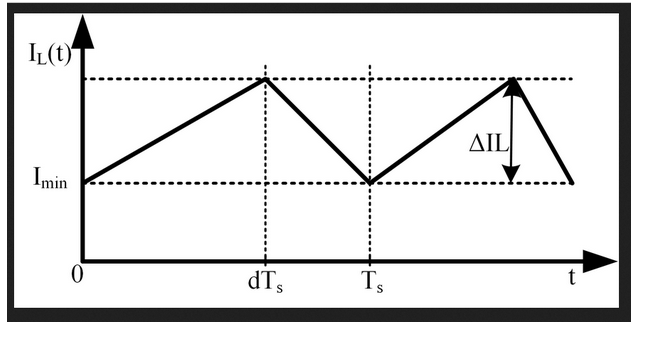
\includegraphics[scale=0.5]{triangular.png}
	\caption{Forma de onda de corriente.}
	\label{fig:img_corriente_triangular}
\end{figure}


----------------------------------

permanecen encendidas las llaves en 
Al controlar el tiempo de activación de las llaves, se podría obtener una forma de onda triangular con un valor medio determinado. Una manera de controlar las llaves es mediante un controlador con histéresis

La etapa de controlador de corriente tiene una tensiòn en su entrada que es tomada como referencia. Es decir, se desea que la corriente del electroimàn sea proporcional a esta tensiòn. Para ello primero se necesita medir la corriente que circula en el elctroimàn, traducirla a una tensiòn para luego esr comparada con esta referemcia. Dependiendo de si una es mayor que la otra, un controlador modifica el estado de las llaves para equiluibrar esta stiuacion. 

Es necesario poder controlar el comportamiento de las llaves para poder manejar cuándo la corriente en el inductor crece y decrece. 

Para poder determinar que llaves encender y cuales apagar, es necesario sabe saber si la corriente debe aumentar o disminuir.

Estas son controladas por un circuito que compara el valor de corriente con una referencia y conmuta las llaves segùn sea necesario.

 manejados por el controlador por histéresis como se observa en la figura \ref{fig:img_topologia-puenteH}. Pueden diferenciarse dos semiciclos de trabajo: uno de estado ON y otro de estado OFF. El primero se define como el semiciclo durante el cual la corriente en el inductor crece (pendiente positiva), mientras que el segundo se da cuando la corriente decrece.

\begin{figure}[H]
	\centering
	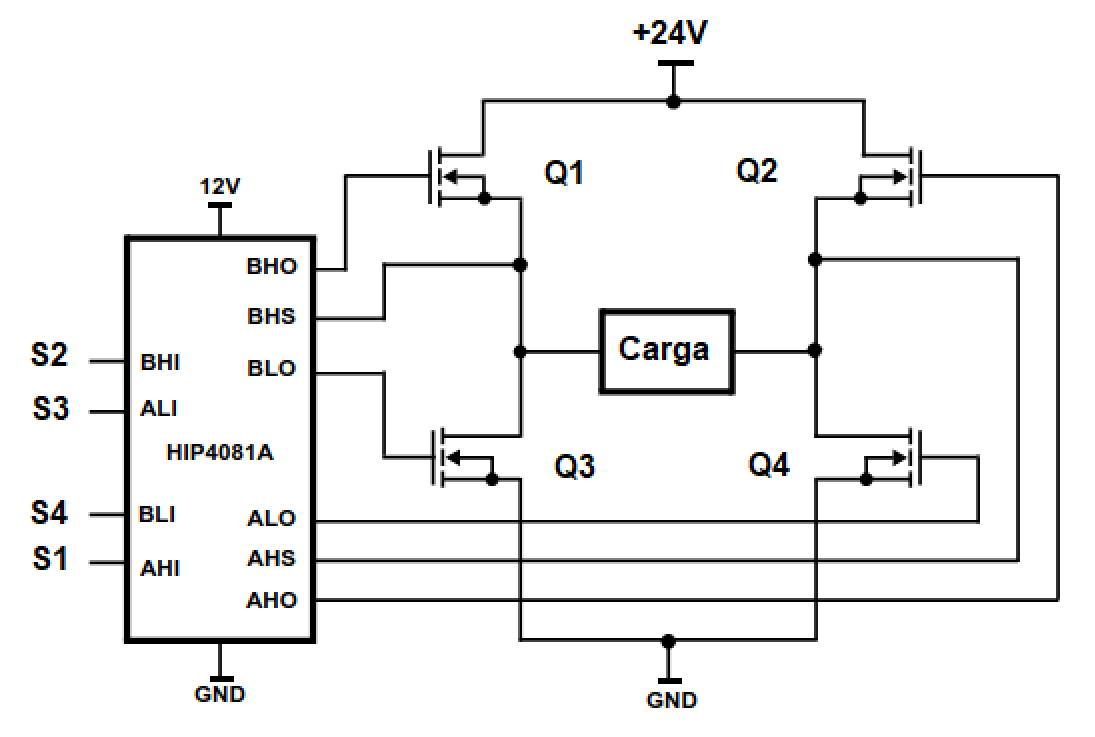
\includegraphics[scale=0.7]{Topologia-puenteH.png}
	\caption{Topología elemental del puente H.}
	\label{fig:img_topologia-puenteH}
\end{figure}
